% Author: Izaak Neutelings (July 2018)
% page 8 https://archive.org/details/StaticAndDynamicElectricity
% https://tex.stackexchange.com/questions/56353/extract-x-y-coordinate-of-an-arbitrary-point-on-curve-in-tikz
% https://tex.stackexchange.com/questions/412899/tikz-calculate-and-store-the-euclidian-distance-between-two-coordinates

\documentclass[border=3pt,tikz]{standalone}
\usepackage{amsmath} % for \dfrac
\usepackage{mathabx} % for \Earth
\usepackage{bm} % \bm
\usepackage{physics}
\usepackage{tikz,pgfplots}
\usepackage[outline]{contour} % glow around text
\usetikzlibrary{angles,quotes} % for pic (angle labels)
\usetikzlibrary{calc}
\usetikzlibrary{decorations.markings}
\tikzset{>=latex} % for LaTeX arrow head
\contourlength{1.6pt}
\usepackage{xcolor}
\colorlet{Ecol}{orange!90!black}
\colorlet{EcolFL}{orange!80!black}
\colorlet{veccol}{green!45!black}
\colorlet{EFcol}{red!60!black}
\tikzstyle{EcolEP}=[blue!80!white]
\tikzstyle{charged}=[top color=blue!30,bottom color=blue!50,shading angle=10]
\tikzstyle{darkcharged}=[very thin,top color=blue!60,bottom color=blue!80,shading angle=10]
\tikzstyle{charge+}=[very thin,top color=red!50,bottom color=red!90!black,shading angle=20]
\tikzstyle{charge-}=[very thin,top color=blue!50,bottom color=blue!80,shading angle=20]
\tikzstyle{gauss surf}=[blue!90!black,top color=blue!2,bottom color=blue!80!black!70,shading angle=5,fill opacity=0.1]
\tikzstyle{gauss line}=[blue!90!black]
\tikzstyle{vector}=[->,thick,veccol]
\tikzset{EFieldLine/.style={thick,EcolFL,decoration={markings,mark=at position #1 with {\arrow{latex}}},
                                 postaction={decorate}},
         EFieldLine/.default=0.5}
\tikzstyle{measure}=[fill=white,midway,outer sep=2]
\def\L{8}
\def\W{0.25}
\def\N{14}


\begin{document}


% E FIELD horizontal, positive charge
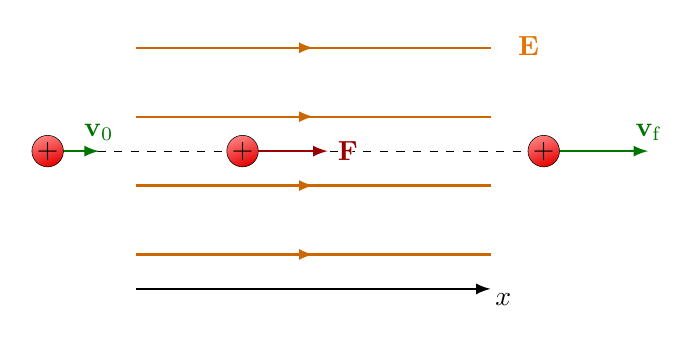
\begin{tikzpicture}
  \def\R{0.2}
  \def\M{4}
  \def\xmax{4.5}
  \def\ymax{3.5}
  \coordinate (Q) at (-0.25*\xmax,0.5*\ymax);
  \coordinate (M) at ( 0.30*\xmax,0.5*\ymax);
  \coordinate (F) at ( 1.15*\xmax,0.5*\ymax);
  
  % ELECTRIC FIELD
  \draw[->,thick] (0,0) -- (\xmax,0) node[below right=-2] {$x$};
  \foreach \i [evaluate={\y=(\i-0.5)*\ymax/\M;}] in {1,...,\M}{
    \draw[EFieldLine] (0,\y) -- (\xmax,\y);
  }
  \node[Ecol,right] at (1.05*\xmax,0.88*\ymax) {$\vb{E}$};
  
  % PATH
  \draw[dashed] (Q) -- (F);
  
  % CHARGE
  \draw[vector]  (Q) ++ (\R,0) --++ (0.1*\xmax,0) node[above] {$\vb{v}_0$};
  \draw[vector,EFcol] (M) --++ (0.24*\xmax,0) node[right] {\contour{white}{$\vb{F}$}};
  \draw[vector]  (F) ++ (\R,0) --++ (0.25*\xmax,0) node[above] {$\vb{v}_\text{f}$};
  
  % CHARGE
  \draw[charge+] (Q) circle (\R) node {$+$};
  \draw[charge+] (M) circle (\R) node {$+$};
  \draw[charge+] (F) circle (\R) node {$+$};
  
\end{tikzpicture}


% E FIELD horizontal, negative charge
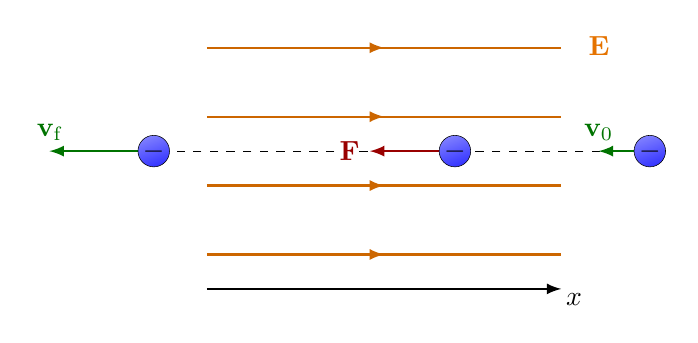
\begin{tikzpicture}
  \def\R{0.2}
  \def\M{4}
  \def\xmax{4.5}
  \def\ymax{3.5}
  \coordinate (Q) at ( 1.25*\xmax,0.50*\ymax);
  \coordinate (M) at ( 0.70*\xmax,0.50*\ymax);
  \coordinate (F) at (-0.15*\xmax,0.50*\ymax);
  
  % ELECTRIC FIELD
  \draw[->,thick] (0,0) -- (\xmax,0) node[below right=-2] {$x$};
  \foreach \i [evaluate={\y=(\i-0.5)*\ymax/\M;}] in {1,...,\M}{
    \draw[EFieldLine] (0,\y) -- (\xmax,\y);
  }
  \node[Ecol,right] at (1.05*\xmax,0.88*\ymax) {$\vb{E}$};
  
  % PATH
  \draw[dashed] (Q) -- (F);
  
  % CHARGE
  \draw[vector]  (Q) ++ (-\R,0) --++ (-0.1*\xmax,0) node[above] {$\vb{v}_0$};
  \draw[vector,EFcol] (M) --++ (-0.24*\xmax,0) node[left] {\contour{white}{$\vb{F}$}};
  \draw[vector]  (F) ++ (-\R,0) --++ (-0.25*\xmax,0) node[above] {$\vb{v}_\text{f}$};
  
  % CHARGE
  \draw[charge-] (Q) circle (\R) node {$-$};
  \draw[charge-] (M) circle (\R) node {$-$};
  \draw[charge-] (F) circle (\R) node {$-$};
  
\end{tikzpicture}


% E FIELD vertical
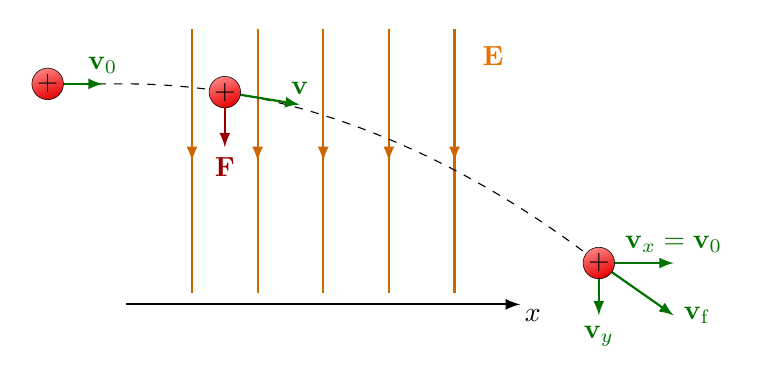
\begin{tikzpicture}
  \def\R{0.2}
  \def\M{5}
  \def\xmax{5.0}
  \def\ymax{3.5}
  \coordinate (Q) at (-0.20*\xmax,0.80*\ymax);
  \coordinate (M) at (+0.25*\xmax,0.77*\ymax);
  \coordinate (F) at (+1.20*\xmax,0.15*\ymax);
  
  % ELECTRIC FIELD
  \draw[->,thick] (0,0) -- (\xmax,0) node[below right=-2] {$x$};
  \foreach \i [evaluate={\x=\i*\xmax/(\M+1);}] in {1,...,\M}{
    \draw[EFieldLine] (\x,\ymax) -- (\x,0.04*\ymax);
  }
  \node[Ecol,right] at (0.88*\xmax,0.9*\ymax) {$\vb{E}$};
  
  % PATH
  \draw[dashed] (Q) -- (0,0.80*\ymax) parabola (F);
  
  % VECTORS
  \draw[vector]  (Q) ++ (\R,0) --++ (0.1*\xmax,0) node[above] {$\vb{v}_0$};
  \draw[vector]  (M) --++ (\R+0.15*\xmax,-0.045*\ymax) node[above] {$\vb{v}$};
  \draw[vector,EFcol] (M) --++ (0,-0.2*\ymax) node[below] {$\vb{F}$};
  \draw[vector]  (F) --++ (\R+0.15*\xmax,0) node[above] {$\vb{v}_x = \vb{v}_0$};
  \draw[vector]  (F) --++ (0,-0.19*\ymax) node[below] {$\vb{v}_y$};
  \draw[vector]  (F) --++ (\R+0.15*\xmax,-0.19*\ymax) node[right] {$\vb{v}_\text{f}$};
  
  % CHARGE
  \draw[charge+] (Q) circle (\R) node {$+$};
  \draw[charge+] (M) circle (\R) node {$+$};
  \draw[charge+] (F) circle (\R) node {$+$};
  
\end{tikzpicture}


% E FIELD vertical - potential
\def\R{0.24}
\def\NE{4}
\def\NQ{7}
\def\xmax{5.0}
\def\ymax{4.1}
\def\a{0.025*\xmax}
\begin{tikzpicture}
  
  \coordinate (P) at (0.50*\xmax,0.81*\ymax);
  \coordinate (A) at (0.23*\xmax,0.81*\ymax);
  \coordinate (B) at (0.23*\xmax,0.26*\ymax);
  
  % ELECTRIC FIELD
  \foreach \i [evaluate={\x=(\i-0.8)*\xmax/(\NE-0.6);}] in {1,...,\NE}{
    \draw[EFieldLine] (\x,\ymax) -- (\x,0);
  }
  \foreach \i [evaluate={\x=(\i-0.5)*\xmax/\NQ;}] in {1,...,\NQ}{
    \node[blue!80!black,scale=0.9] at (\x,-0.04*\ymax) {$-$};
  }
  \node[Ecol] at (1.02*\xmax,0.65*\ymax) {$\vb{E}$};
  
  % BOTTOM CHARGE
  \draw[blue!80!black,thick] (0,0) -- (\xmax,0);
  \fill[top color=blue!50,bottom color=white,shading angle=0] (0,0) rectangle ++(\xmax,-0.20*\ymax);
  \node[blue!80!black] at (0.5*\xmax,-0.11*\ymax) {$-Q$};
  
  % CHARGE
  \draw[vector,EFcol] (P) --++ (0,-0.3*\ymax) node[below] {$\vb{F} = q\vb{E}$}; %{\contour{white}{$\vb{F} = q\vb{E}$}};
  \draw[charge+] (P) circle (\R) node[scale=0.85] {$+q$};
  
  % AXIS
  \draw[thin] (A) --++ (\a,0) --++ (-2*\a,0) node[left] {$a$};
  \draw[thin] (B) --++ (\a,0) --++ (-2*\a,0) node[left] {$b$};
  \draw[->] (A) -- (B) node[midway] {\contour{white}{$d$}};
  
\end{tikzpicture}


% G FIELD vertical - potential
\begin{tikzpicture}
  
  \coordinate (P) at (0.50*\xmax,0.81*\ymax);
  \coordinate (A) at (0.23*\xmax,0.81*\ymax);
  \coordinate (B) at (0.23*\xmax,0.26*\ymax);
  
  % ELECTRIC FIELD
  \foreach \i [evaluate={\x=(\i-0.8)*\xmax/(\NE-0.6);}] in {1,...,\NE}{
    \draw[EFieldLine] (\x,\ymax) -- (\x,0);
  }
  \node[Ecol] at (1.02*\xmax,0.65*\ymax) {$\vb{g}$};
  
  % EARTH
  \draw[brown!40!black!90,thick] (0,0) -- (\xmax,0);
  \fill[top color=green!50!black!80,bottom color=white,shading angle=0] (0,0) rectangle ++(\xmax,-0.20*\ymax);
  \node[brown!40!black] at (0.5*\xmax,-0.11*\ymax) {Earth, $M_\Earth$};
  
  % CHARGE
  \draw[vector,EFcol] (P) --++ (0,-0.3*\ymax) node[below] {$\vb{F} = m\vb{g}$}; %{\contour{white}{$\vb{F} = q\vb{E}$}};
  \draw[charge+] (P) circle (\R) node[scale=0.9] {$m$};
  
  % AXIS
  \draw[thin] (A) --++ (\a,0) --++ (-2*\a,0) node[left] {$a$};
  \draw[thin] (B) --++ (\a,0) --++ (-2*\a,0) node[left] {$b$};
  \draw[->] (A) -- (B) node[midway] {\contour{white}{$h$}};
  
\end{tikzpicture}


% PATH INTEGRATION
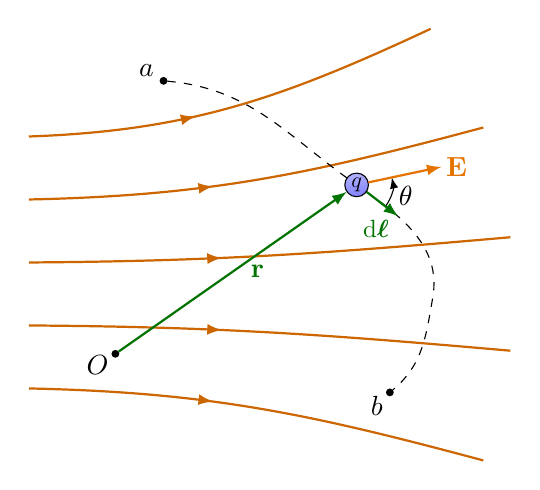
\begin{tikzpicture}
  \def\N{5}
  \def\R{2.2}
  \def\E{6.8}
  \def\r{0.85}
  \node[circle,fill=black,inner sep=1,outer sep=0] (O) at (0,0) {};
  \node[circle,fill=black,inner sep=1,outer sep=0] (A) at (80:1.6*\R) {};
  \coordinate (B) at (10:1.86*\R) {};
  \node[circle,fill=black,inner sep=1,outer sep=0] (C) at (-8:1.6*\R) {};
  \coordinate (P) at (35:1.7*\R);
  \coordinate (L) at ($(P)+(-37:0.30*\R)$);
  \coordinate (E) at ($(P)+(12:0.5*\R)$);
  
  % FIELD LINES
  \begin{scope}[shift={(0.90*\R,0.6*\R)}]
    \foreach \i [evaluate={
        \y=0.8*(\i-0.7-\N/2);
        \ang=6*(\i-\N/2);    \r=2.8*\R-0.14*(\i-\N/2)^2;
        \out=0.8*(\i-\N/2);  \in=180+10*(\i-\N/2);
      }] in {1,...,\N}{
      \draw[EFieldLine={0.4}] (-1.4*\R,\y) to[out=\out,in=\in]++ (\ang:\r);
    }
  \end{scope}
  
  % PATH
  %\draw[->] (O) -- (A) node[midway,fill=white,inner sep=1] {$r_a$} node[above left=-2] {$a$};
  %\draw[->] (O) -- (C) node[midway,fill=white,inner sep=1] {$r_b$} node[left=2,below right=-1] {$b$};
  \node[below=2,above left=0] at (A) {$a$};
  \node[left=1,below left=-2] at (C) {$b$};
  \draw[thin,dashed] (A) to[out=-5,in=145] (P) to[out=-35,in=80] (B) to[out=-100,in=40] (C);
  \node[charged,draw=black,circle,inner sep=1,black,scale=0.8] (Q) at (P) {$q$};
  \draw[vector] (O) -- (Q) node[midway,right=9,below=-6] {$\vb{r}$};
  \draw pic[->,"$\theta$",draw=black,angle radius=13,angle eccentricity=1.4] {angle = L--Q--E};
  \draw[vector] (Q.-35) -- (L) node[left=2,below left=-2,scale=0.9] {$\dd{\bm{\ell}}$};
  \draw[vector,Ecol] (Q) -- (E) node[right=-2] {$\vb{E}$};
  \node[above=2,below left=-1] at (O) {$O$};
  %\draw (0,0) -- (B);
  
\end{tikzpicture}


% E FIELD horizontal, work
\def\R{0.2}
\def\a{0.025*\xmax}
\def\M{2}
\def\xmax{3.6}
\def\ymax{1.4}
\begin{tikzpicture} % q>0, E.dl>0
  \coordinate (P) at ( 0.20*\xmax,0.65*\ymax);
  \coordinate (A) at ( 0.20*\xmax,0.4*\ymax);
  \coordinate (B) at ( 0.80*\xmax,0.4*\ymax);
  \draw[EFieldLine] (0,0) --++ (\xmax,0);
  \draw[EFieldLine] (0,\ymax) --++ (\xmax,0) node[Ecol,above=1,right=2] {$\vb{E}$};
  \draw[vector,EFcol] (P) --++ (0.24*\xmax,0) node[right] {$\vb{F}$};
  \draw[charge+] (P) circle (\R) node {$+$};
  \draw[thin] (A) --++ (0,\a) --++ (0,-2*\a) node[below] {$a$};
  \draw[thin] (B) --++ (0,\a) --++ (0,-2*\a) node[below=-2] {$b$};
  \draw[vector] (A) -- (B) node[midway,below=-1] {$\bm{\Delta\ell}$};
\end{tikzpicture}
\begin{tikzpicture} % q>0, E.dl<0
  \coordinate (P) at ( 0.80*\xmax,0.65*\ymax);
  \coordinate (A) at ( 0.80*\xmax,0.4*\ymax);
  \coordinate (B) at ( 0.20*\xmax,0.4*\ymax);
  \draw[EFieldLine] (0,0) --++ (\xmax,0);
  \draw[EFieldLine] (0,\ymax) --++ (\xmax,0) node[Ecol,above=1,right=2] {$\vb{E}$};
  \draw[vector,EFcol] (P) --++ (0.24*\xmax,0) node[right] {$\vb{F}$};
  \draw[charge+] (P) circle (\R) node {$+$};
  \draw[thin] (A) --++ (0,\a) --++ (0,-2*\a) node[below] {$a$};
  \draw[thin] (B) --++ (0,\a) --++ (0,-2*\a) node[below=-2] {$b$};
  \draw[vector] (A) -- (B) node[midway,below=-1] {$\bm{\Delta\ell}$};
\end{tikzpicture}
\begin{tikzpicture} % q<0, E.dl<0
  \coordinate (P) at ( 0.80*\xmax,0.65*\ymax);
  \coordinate (A) at ( 0.80*\xmax,0.4*\ymax);
  \coordinate (B) at ( 0.20*\xmax,0.4*\ymax);
  \draw[EFieldLine] (0,0) --++ (\xmax,0);
  \draw[EFieldLine] (0,\ymax) --++ (\xmax,0) node[Ecol,above=1,right=2] {$\vb{E}$};
  \draw[vector,EFcol] (P) --++ (-0.24*\xmax,0) node[left] {$\vb{F}$};
  \draw[charge-] (P) circle (\R) node {$-$};
  \draw[thin] (A) --++ (0,\a) --++ (0,-2*\a) node[below] {$a$};
  \draw[thin] (B) --++ (0,\a) --++ (0,-2*\a) node[below=-2] {$b$};
  \draw[vector] (A) -- (B) node[midway,below=-1] {$\bm{\Delta\ell}$};
\end{tikzpicture}
\begin{tikzpicture} % q<0, E.dl>0
  \coordinate (P) at ( 0.20*\xmax,0.65*\ymax);
  \coordinate (A) at ( 0.20*\xmax,0.4*\ymax);
  \coordinate (B) at ( 0.80*\xmax,0.4*\ymax);
  \draw[EFieldLine] (0,0) --++ (\xmax,0);
  \draw[EFieldLine] (0,\ymax) --++ (\xmax,0) node[Ecol,above=1,right=2] {$\vb{E}$};
  \draw[vector,EFcol] (P) --++ (-0.24*\xmax,0) node[left] {$\vb{F}$};
  \draw[charge-] (P) circle (\R) node {$-$};
  \draw[thin] (A) --++ (0,\a) --++ (0,-2*\a) node[below] {$a$};
  \draw[thin] (B) --++ (0,\a) --++ (0,-2*\a) node[below=-2] {$b$};
  \draw[vector] (A) -- (B) node[midway,below=-1] {$\bm{\Delta\ell}$};
\end{tikzpicture}


% E FIELD horizontal, potential
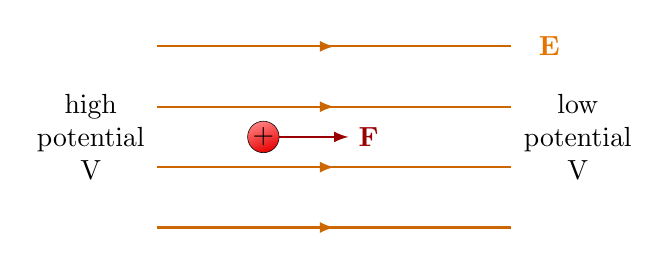
\begin{tikzpicture}
  \def\R{0.2}
  \def\M{4}
  \def\xmax{4.5}
  \def\ymax{2.3}
  \coordinate (P) at ( 0.30*\xmax,0.5*\ymax);
  
  % ELECTRIC FIELD
  \foreach \i [evaluate={\y=(\i-1)*\ymax/(\M-1);}] in {1,...,\M}{
    \draw[EFieldLine] (0,\y) -- (\xmax,\y);
  }
  \node[Ecol,right] at (1.05*\xmax,\ymax) {$\vb{E}$};
  \node[left=1,align=center] at (0,\ymax/2) {high\\potential\\V};
  \node[right=1,align=center] at (\xmax,\ymax/2) {low\\potential\\V};
  
  % CHARGE
  \draw[vector,EFcol] (P) --++ (0.24*\xmax,0) node[right] {\contour{white}{$\vb{F}$}};
  \draw[charge+] (P) circle (\R) node {$+$};
  
\end{tikzpicture}


% E FIELD horizontal, equipotential
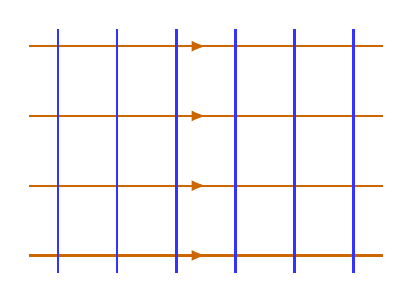
\begin{tikzpicture}
  \def\R{0.2}
  \def\NE{4}
  \def\NQ{6}
  \def\xmax{4.5}
  \def\ymax{3.1}
  \coordinate (P) at ( 0.30*\xmax,0.5*\ymax);
  
  % ELECTRIC FIELD
  \foreach \i [evaluate={\y=(\i-0.75)*\ymax/(\NE-0.5);}] in {1,...,\NE}{
    \draw[EFieldLine] (0,\y) -- (\xmax,\y);
  }
  \foreach \i [evaluate={\x=(\i-0.5)*\xmax/\NQ;}] in {1,...,\NQ}{
    \draw[EcolEP,thick] (\x,0) --++ (0,\ymax);
  }
  %\node[Ecol,right] at (1.05*\xmax,\ymax) {$\vb{E}$};
  
\end{tikzpicture}


\end{document}
